%
% section 2.5
%
\setcounter{section}{4}
\section{Ασύρματα Δίκτυα}
Σε ένα ασύρματο δίκτυο, αντί για καλώδιο το μέσο διάδοσης είναι ο αέρας (ή και το κενό). Για τη μετάδοση χρησιμοποιούνται οπτικά σήματα, υπέρυθρες, ή (συνηθέστερα) ραδιοκύματα. 

Τα ασύρματα δίκτυα με τη μεγαλύτερη εξάπλωση σήμερα είναι τα κυψελοειδή: πολλά από τα ασύρματα συστήματα αποτελούν εξειδίκευση ή γενίκευση των κυψελοειδών δικτύων. Κάθε δίκτυο καλύπτει μια περιοχή που ονομάζεται \emph{κυψέλη} χρησιμοποιώντας ένα \emph{σταθμό βάσης} και πολλούς ασύρματους \emph{χρήστες -- δέκτες}. 

Κάθε κυψέλη καλύπτει με σήμα μια περίπου εξαγωνική ή κυκλική περιοχή. Πολλές κυψέλες μαζί καλύπτουν ασύρματα μεγάλες εκτάσεις, όπως φαίνεται στο σχήμα \ref{2-6}.

\begin{figure}[!ht]
  \centering
  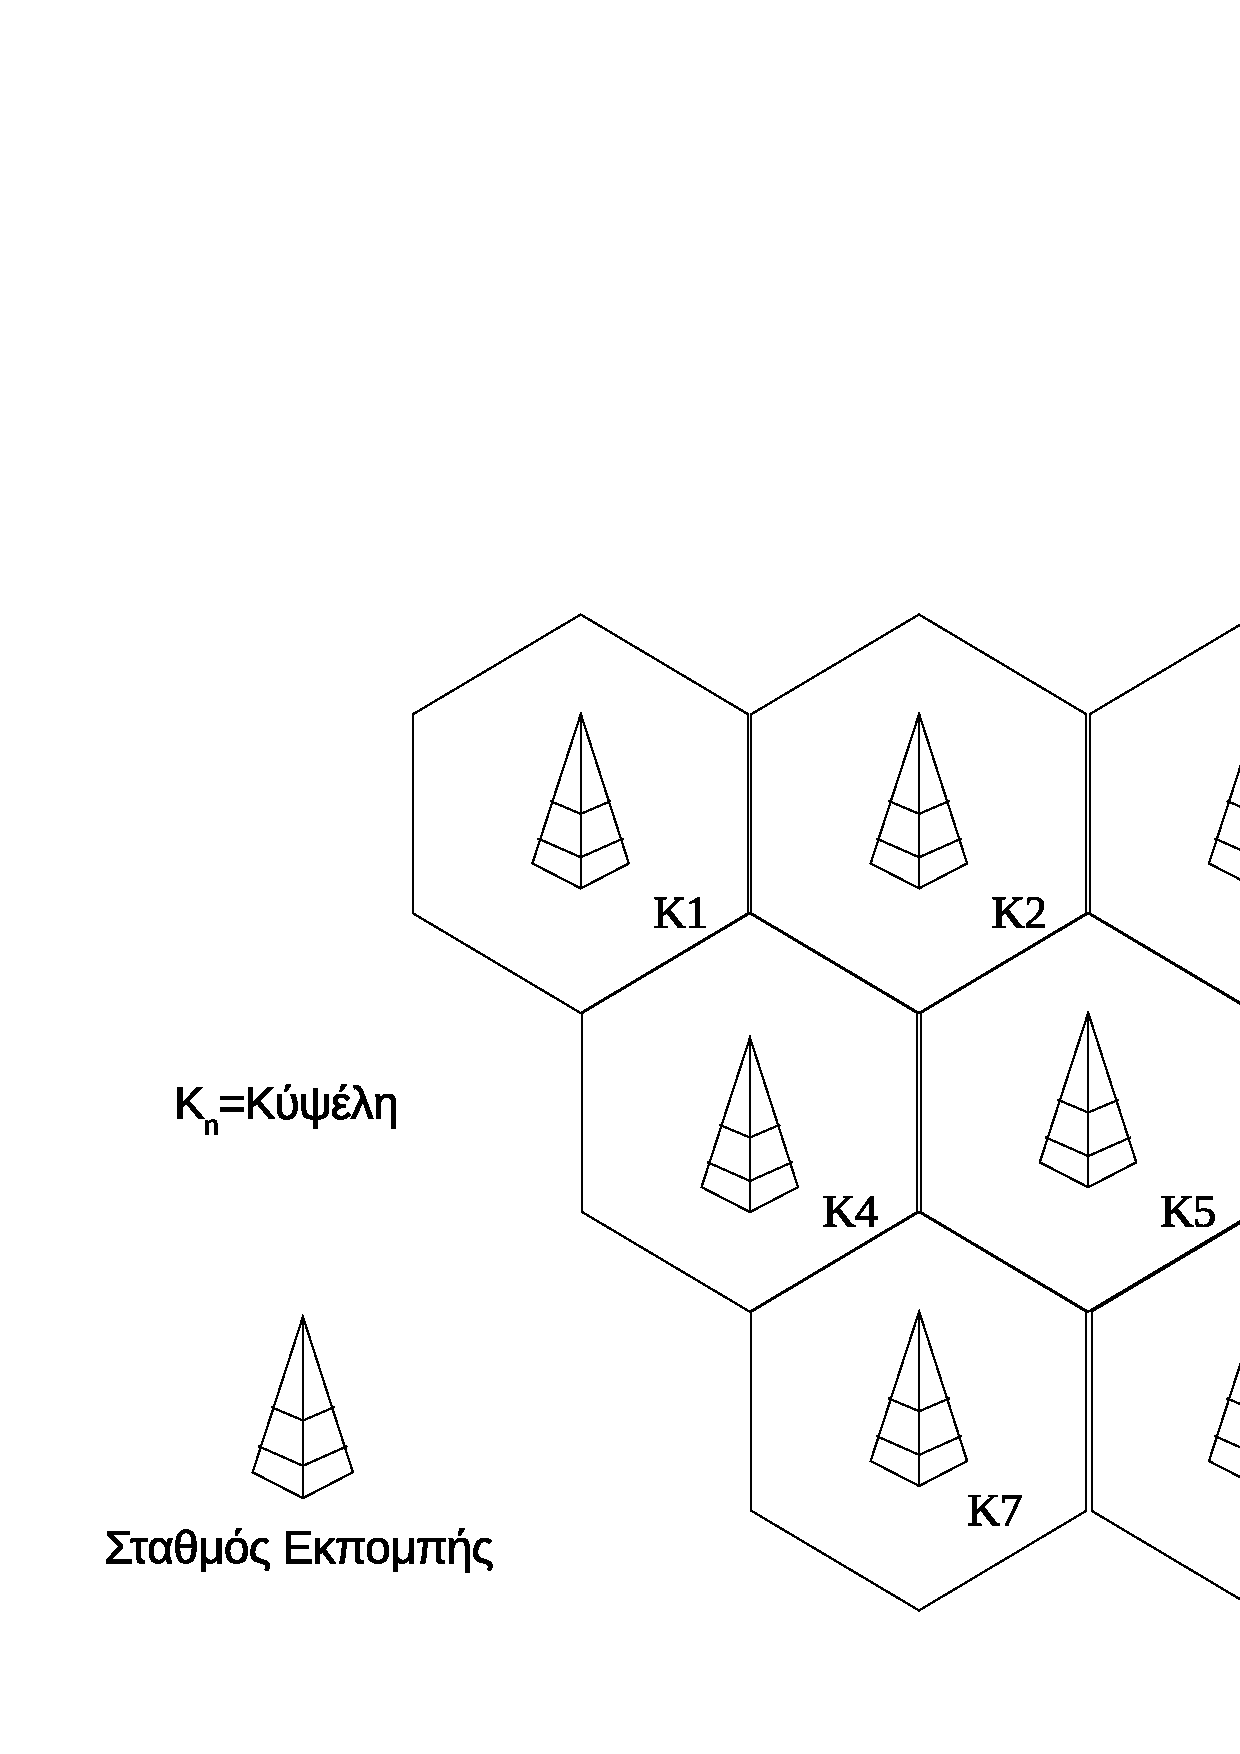
\includegraphics[width=0.90\textwidth]{images/chapter2/2-6}
  \caption {\textsl{Δίκτυο με Κυψέλες}}
  \label{2-6}
\end{figure}

Προϋπόθεση για τη σύνδεση των συσκευών μεταξύ τους είναι να έχουν εξοπλιστεί με κατάλληλο υλικό διεπαφής (π.χ. ασύρματες κάρτες δικτύου) που να επιτρέπει τη σύνδεση τους μέσω ασύρματης τεχνολογίας.

\parbox{\textwidth}{
\boxline
\textbf{Ένα καθημερινό παράδειγμα δικτύου με κυψέλες}\\

Ένα είδος ασύρματου δικτύου που χρησιμοποιεί κυψέλες είναι και το σύστημα κινητής τηλεφωνίας (GSM). Κάθε φορητή συσκευή (κινητό τηλέφωνο) είναι εφοδιασμένη με τον κατάλληλο πομποδέκτη και κυκλώματα που αφορούν τη ψηφιοποίηση των δεδομένων φωνής. Ο πάροχος της υπηρεσίας διαθέτει κυψέλες που γεωγραφικά καλύπτουν ολόκληρη τη χώρα. Καθώς το κινητό τηλέφωνο μετακινείται, συνδέεται κάθε φορά στην πιο κοντινή/ισχυρή κυψέλη χωρίς ο χρήστης να αντιλαμβάνεται τη μετάβαση από τη μια κυψέλη στην άλλη.\\
\boxline}

Τα \textbf{ασύρματα τοπικά δίκτυα} ή WLAN (Wireless Local Area Network) επιτρέπουν σε ένα χρήστη κινητής συσκευής όπως ένας φορητός υπολογιστής, tablet ή smartphone να συνδέονται σε ένα τοπικό δίκτυο μέσω ασύρματης σύνδεσης ραδιοκυμάτων υψηλής συχνότητας.

\begin{figure}[!ht]
  \centering
  \includegraphics[width=0.65\textwidth]{images/chapter2/2-7}
  \caption {\textsl{Ασύρματο τοπικό δίκτυο συνδεόμενο με ενσύρματο δίκτυο}}
  \label{2-7}
\end{figure}

Στο σχήμα \ref{2-7} φαίνεται ένα τέτοιο δίκτυο που αποτελείται από τρία σημεία πρόσβασης (APs, Access Points) τα οποία σχηματίζουν ένα τοπικό ασύρματο δίκτυο και επιτρέπουν σε φορητές συσκευές που βρίσκονται στην εμβέλεια τους να συνδεθούν σε αυτά. Τα σημεία πρόσβασης συνδέονται μεταξύ τους και με το υπόλοιπο δίκτυο μέσω ενός μεταγωγέα (switch). Με αυτό το τρόπο δίνεται η δυνατότητα επέκτασης του τοπικού δικτύου και παροχής υπηρεσιών σε μεγαλύτερο αριθμό συσκευών. 

Το \textbf{Πρωτόκολλο IEEE 802.11} υλοποιεί τα ασύρματα τοπικά δίκτυα. Το πρωτόκολλο αυτό διαιρείται σε μια ομάδα προτύπων ασύρματης δικτύωσης  τα οποία χαρακτηρίζονται με τα γράμματα από το `a' ως το `n' (π.χ. 802.11n) και τα οποία αποτελούν τα παγκοσμίως επικρατέστερα πρότυπα. Το 802.11 περιγράφει τα δύο κατώτερα επίπεδα του OSI (φυσικό και σύνδεσης δεδομένων) και μπορεί να λειτουργήσει με οποιεσδήποτε συσκευές ακολουθούν το πρότυπο OSI. Ουσιαστικά το 802.11 μεταφέρει την πληροφορία από και προς τα ανώτερα επίπεδα του OSI. Το 802.11 χρησιμοποιεί τεχνολογίες αντίστοιχες με το Ethernet και επιτρέπει την πολλαπλή πρόσβαση στο μέσο με την τεχνική CSMA/CA  (Carrier Sense Multiple Access with Collision Avoidance). Καθώς τα δεδομένα μεταδίδονται στον αέρα και μπορούν να ληφθούν από τον καθένα, χρησιμοποιείται κρυπτογράφηση, με  γνωστότερους τους αλγόριθμους WEP, WPA, WPA2 (το WEP είναι ξεπερασμένο και ανασφαλές).

Μερικές γνωστές παραλλαγές του 802.11 φαίνονται παρακάτω:

\begin{center}
\begin{tabular}{|c|c|c|}
  \hline
    \textbf{Πρότυπο ΙΕΕΕ}&\textbf{Μέγιστος Ρυθμός Μετάδοσης}&\textbf{Συχνότητες}\\
  \hline
  \textbf{802.11} & 1 Mbps / 2 Mbps & 2.4 GHz \\
  \hline
  \textbf{802.11a} & 11 Mbps & 5 GHz \\
  \hline
  \textbf{802.11b} & 5.5 Mbps / 11 Mbps & 2.4 GHz \\
  \hline
  \textbf{802.11g} & 54 Mbps & 2.4 GHz \\
  \hline
  \textbf{802.11n} & 600 Mbps & 2.4 GHz και 5 GHz \\
  \hline
\end{tabular}
\end{center}

\begin{inthebox}
Ένα \textbf{Ασύρματο Σημείο Πρόσβασης} (Access Point, AP) είναι μια συσκευή που αναλαμβάνει την επικοινωνία μέσω ραδιοκυμάτων με τους ασύρματους σταθμούς μιας κυψέλης. Ουσιαστικά παίζει το ρόλο που παίζει ένα switch σε ένα δίκτυο Ethernet. Το Access Point συχνά είναι μια αυτόνομη εξωτερική συσκευή και μπορεί να συνδέεται ενσύρματα με ένα δρομολογητή.  Συχνά επίσης περιέχεται μέσα στους οικιακούς ADSL modems/routers με τους οποίους συνδεόμαστε στο Internet. Τέλος μπορεί να υλοποιηθεί και μια εσωτερική ή εξωτερική ασύρματη κάρτα δικτύου και κατάλληλο λογισμικό σε ένα υπολογιστή.\\
\end{inthebox} 

Το σημείο πρόσβασης λειτουργεί ως σταθμός βάσης, συγκεντρώνοντας την κίνηση από τους ασύρματους σταθμούς και κατευθύνοντας την προς το υπόλοιπο δίκτυο. Επίσης περιλαμβάνει λειτουργίες αυθεντικοποίησης για την σύνδεση και συσχέτιση ενός νέου σταθμού εργασίας στο ασύρματο δίκτυο.